\documentclass[11pt]{article}

% ── Encoding ──
\usepackage[utf8]{inputenc}
\usepackage[T1]{fontenc}

% ── Professional preprint style (shared arxiv.sty template):
%    Palatino body + matching math, Helvetica-clone sans headings, a ruled
%    centred title block, and a slim running header. It also provides page
%    geometry, so no separate geometry package is loaded here.
\usepackage{arxiv}

% ── Content packages ──
\usepackage{natbib}
\usepackage{url}
\usepackage{booktabs}
\usepackage{array}
\usepackage{amsmath,amssymb}
\usepackage{graphicx}
\usepackage{xcolor}
\usepackage{tcolorbox}
\tcbuselibrary{skins,breakable}
\usepackage{caption}
\captionsetup{font=small,labelfont=bf}

% ── hyperref loaded late, then coloured to match the palette ──
\usepackage{hyperref}
\hypersetup{
  colorlinks=true,
  linkcolor=arxivaccent,
  citecolor=arxivaccent,
  urlcolor=arxivaccent,
  filecolor=arxivaccent,
  breaklinks=true,
}

\graphicspath{{figures/}}

\newcommand{\fire}{\texttt{<END\_SPEECH>}}
\newcommand{\eager}{\texttt{<EAGER\_END\_SPEECH>}}
\newcommand{\ctx}{\texttt{<CTX>}}

% Model names (supervision-descriptive; no internal codenames anywhere).
\newcommand{\moffline}{\mbox{offline-labeled}}
\newcommand{\mmixed}{\mbox{mixed-pools}}
\newcommand{\mopposed}{\mbox{opposed-pools}}
\newcommand{\mcausal}{\mbox{causal}}

\title{Clairvoyant Labels: How Offline Supervision Manufactures\\ Phantom Trade-offs in Streaming Models}

% Author email (not for publication): Noah Shi <noahshi@cs.washington.edu>
\author{%
  \begin{tabular}{@{}c@{\hspace{4em}}c@{}}
    Bojie Li & Noah Shi \\
    Pine AI & University of Washington
  \end{tabular}%
}
\date{}
\runningtitle{Clairvoyant labels manufacture phantom trade-offs in streaming models}

\begin{document}
\maketitle

\begin{abstract}
Streaming models must act on the prefix of their input, but their supervision is routinely manufactured from offline data in which the future is already written. We name the resulting hazard \emph{clairvoyant labels}: training or evaluation targets whose correct value depends on input that arrives \emph{after} the decision point. Because the dependence is systematic rather than random, clairvoyant labels partition training data into internally consistent pools with incompatible optima, and they leave two observable fingerprints: training-time oscillation between mode attractors, and \emph{phantom trade-offs} --- apparent Pareto frontiers across checkpoints that no property of the task enforces. We document this failure mode end-to-end in \emph{turn-aware streaming ASR}: a single model that transcribes while deciding, from semantics and silence jointly, whether the user's turn is over --- a class whose commercial members (Deepgram Flux, OpenAI's semantic VAD) are closed, with no published training account. Across eight successive supervision recipes on a fixed small open model (Qwen3-ASR-0.6B, LoRA, ${\sim}12$k synthesized examples, one GPU), offline-derived labels manufactured exactly these artifacts, and intervention experiments pin the cause to two label-side mechanisms: evaluation clips cut at the end of speech, and pause labels keyed on who speaks next. Rebuilding the data under a single rule --- \textbf{every label must be computable from the causal prefix} --- with architecture, recipe, and scale unchanged eliminates the oscillation and yields one checkpoint that dominates all eight predecessors on a deployment-matched streaming benchmark: 0.97 boundary recall at 0.39\,s median latency with 0.3 false fires per speech-minute. Silence-timeout cascades, the deployed alternative, need $3\times$ the latency and $5\times$ the false fires to match that recall. The released model also carries measured capabilities its base model never published --- a context prefix lifts hotword recall by $+28.9$\,pp, durable across session length --- at a measured, ablation-attributed cost. The diagnosis is not specific to speech: any streaming decision trained on offline-labeled data can inherit it.
\end{abstract}

\begin{center}
\small
Code: \url{https://github.com/19PINE-AI/turn-aware-asr} \quad\textbar\quad Website: \url{https://01.me/research/turn-aware-asr}
\end{center}
\vspace{-0.6em}

\section{Introduction}
\label{sec:intro}

A growing family of models must act \emph{mid-stream}: decide now, on the prefix of an unbounded input, and live with the decision. End-of-turn detection for voice agents, barge-in, read/write decisions in simultaneous translation, action timing for agents --- in each, the model at time $t$ sees only what has arrived by $t$. Its supervision, however, is almost never born streaming. Labels are minted from offline corpora, replayed logs, and completed episodes, in which the future of every decision point is already on disk, and it is easy --- almost default --- for that future to leak into the targets. This paper is about what happens when it does, how to recognize it from the training run alone, and how cheap the repair is once the leak is named.

We call the hazard a \textbf{clairvoyant label}: a target for a decision at time $t$ whose correct value depends on input after $t$ (\S\ref{sec:clair}). A clairvoyant label is not ordinary noise. Because the future-dependence is systematic --- an artifact of how a corpus was cut, or of which outcome happened to follow --- it splits the training data into internally consistent pools whose optimal policies contradict each other on causally identical prefixes. A model trained on such a mixture is not underfitting; it is faithfully fitting a contradiction. We identify two fingerprints that the contradiction leaves in plain sight. During training, holdout accuracy \emph{oscillates} between mode attractors, each satisfying one pool at the expense of the other (Figure~\ref{fig:oscillation}, left). Across checkpoints, capabilities appear to trade off against each other along a frontier that dissolves the moment the labels are made causal (Figure~\ref{fig:oscillation}, right) --- a \emph{phantom} frontier, manufactured by measurement, in the same family of artifacts as metric-induced ``emergence'' \citep{schaeffer2023mirage}.

\begin{figure}[t]
  \centering
  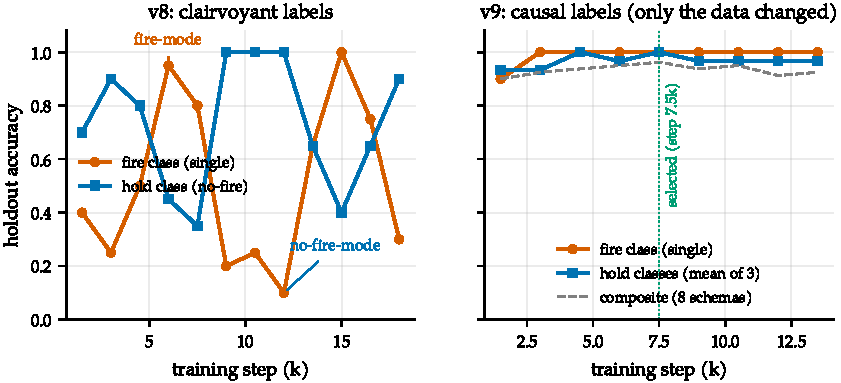
\includegraphics[width=\linewidth]{fig1_oscillation}
  \caption{\textbf{The fingerprint of contradictory supervision.} Left: under opposed-pools supervision (clairvoyant labels; \S\ref{sec:phantom}), holdout accuracy oscillates for the entire run between a \emph{fire-mode} attractor (fire class ${\approx}1.0$, hold class ${\approx}0.4$) and a \emph{no-fire-mode} attractor (fire ${\approx}0.1$, hold ${\approx}1.0$): the training pools assign opposite targets to causally identical audio, so no single policy satisfies both, and optimization circulates between the modes. Right: causal supervision --- same architecture, same LoRA recipe, same data volume, \emph{only the labels changed} --- climbs monotonically, and both classes sit at ceiling \emph{simultaneously} from step 3k on.}
  \label{fig:oscillation}
\end{figure}

Our evidence is a complete, instrumented case study in \textbf{turn-aware streaming ASR}. Every voice interface must answer one deceptively hard question in real time --- \emph{has the user finished talking?} --- and frontier commercial systems have moved that decision \emph{into} the recognizer: Deepgram's Flux emits \texttt{EagerEndOfTurn} events from the ASR model itself \citep{deepgram2026flux}, and OpenAI's Realtime API offers a \texttt{semantic\_vad} mode \citep{openai2025semanticvad}. Every member of the class is closed --- no weights, no recipe, no account of what makes the training work. We build one in the open (Qwen3-ASR-0.6B \citep{qwen3asr2026}, LoRA-fine-tuned to emit an end-of-turn marker inside its transcription stream, trained on one GPU from ${\sim}12$k synthesized examples) and, in doing so, run into the failure mode this paper is about --- at, we believe, exactly the place the closed builders each ran into it privately.

Eight successive supervision recipes, all on the same architecture, traced out what looked like a fundamental trade-off (\S\ref{sec:phantom}, Table~\ref{tab:composition}): checkpoints that fired promptly at turn ends also fired spuriously mid-utterance; checkpoints that never fired spuriously would not fire at all; training runs oscillated between the two behaviors. The project record at the eighth iteration concluded the behaviors lay on a Pareto frontier and recommended shipping two checkpoints, one per deployment. The frontier was a mirage, and we can show the mechanism with interventions rather than forensics: appending one second of deployment-realistic silence to the evaluation clips --- restoring the future that deployment always delivers --- takes the ``broken'' checkpoint's fire recall from 0.10 to 1.00 while leaving a control model untouched (Table~\ref{tab:silappend}); and rebuilding the training pools under a single causal rule, with everything else frozen, removes the oscillation and the trade-off at once (\S\ref{sec:relabel}).

The repaired model is not just a cleaner training curve. On a deployment-matched streaming benchmark (\S\ref{sec:eval}) it dominates all eight predecessors on every axis simultaneously --- 0.97 boundary recall at 0.39\,s median latency with 0.3 false fires per speech-minute, no inference-time crutches --- and it escapes the latency-vs-false-fire curve that the deployed VAD-plus-timeout cascade family is confined to (Figure~\ref{fig:tradeoff}): a silence timeout needs $3\times$ the latency and $5\times$ the false fires to match that recall. A fresh, $2\times$-larger test set drawn after all development ended confirms the operating point (\S\ref{sec:results}).

Our contributions:
\begin{enumerate}\itemsep2pt
  \item \textbf{A named, testable failure mode} (\S\ref{sec:clair}): clairvoyant labels --- a definition, two general mechanisms by which offline-derived supervision demands clairvoyance from streaming models, and the two observable fingerprints they produce (training-time mode oscillation; phantom cross-checkpoint trade-offs).
  \item \textbf{A controlled anatomy} (\S\ref{sec:phantom}): eight supervision compositions on a fixed architecture, presented as a dose--response study of contradiction; a natural experiment separating how contradictions on \emph{identical} versus \emph{distributionally identical} inputs express themselves (collapse versus oscillation); and a one-variable eval intervention that falsifies the frontier.
  \item \textbf{A causal label recipe} (\S\ref{sec:relabel}) whose minimal-pair construction turns the former contradiction into the intended discriminative feature, yielding 0.97 recall at 0.39\,s P50 and 0.3 false fires/min --- confirmed on a fresh $2\times$-larger test set (0.92 recall, 0.42\,s, 0.2 false/min).
  \item \textbf{A deployment-matched streaming benchmark} (\S\ref{sec:eval}): replayed real conversational timelines with a causally-decidable boundary taxonomy. Under it the historical ranking \emph{inverts} (Figure~\ref{fig:inversion}), and a universal blind spot surfaces: every clairvoyantly-supervised model hallucinates on silence-initial audio (Figure~\ref{fig:silence}).
  \item \textbf{An open turn-aware streaming ASR system} (\S\ref{sec:model}, \S\ref{sec:capability}, \S\ref{sec:serving}): weights, recipe, and benchmark released; context biasing measured where its base model published nothing ($+28.9$\,pp on Earnings-22, flat across session age); the fine-tune's offline WER cost measured \emph{and attributed} by ablation; the whole system running on stock vLLM at 84\,ms per 0.5\,s chunk.
\end{enumerate}

Section~\ref{sec:checklist} compresses the lesson into a four-question checklist. The pattern --- offline-labeled data supervising an online decision --- recurs in dialogue turn-taking, barge-in, simultaneous translation, streaming TTS, and agent action-timing. We suspect phantom frontiers are being chased in several of these right now.

%% TODO(exp-1): multi-seed replication of opposed-pools vs causal (>=3 seeds each): does the
%%   oscillation always appear under contradictory pools and never under causal labels?
%%   Turns Fig 1 from one run per condition into a reproducible phenomenon with error bars.
%% TODO(exp-5): synthetic streaming-decision toy task with a dialable contradiction rate
%%   (oscillation amplitude / frontier width vs contradiction fraction). Cheapest path to
%%   generality beyond speech; would slot in as a new subsection at the end of Sec. 2.

\section{Clairvoyant labels}
\label{sec:clair}

\paragraph{Setup.} A streaming decision task presents input $x_{1:T}$ incrementally. At each step $t$ a policy must choose an action $a_t$ --- here, binary: \emph{fire} an irreversible event or \emph{hold} --- using only the prefix $x_{\le t}$. Supervision supplies example streams with target actions $y_t$. Nothing in this setup is exotic; what is easy to miss is a measurability requirement on the \emph{labels}:

\begin{tcolorbox}[title=\textbf{Clairvoyant labels},colback=red!3!white,colframe=red!50!black]
A label for a streaming decision at time $t$ is \emph{clairvoyant} if its value depends on input after $t$. Pools containing clairvoyant labels do not merely add noise: because the dependence is systematic, they partition the data into internally consistent subsets with incompatible optima. The observable symptoms are (a)~training-time oscillation between mode attractors and (b)~apparent capability trade-offs across checkpoints --- a phantom Pareto frontier. \textbf{Principle: every training label and every evaluation target for a streaming decision must be computable from the causal prefix.}
\end{tcolorbox}

\paragraph{Why contradiction rather than noise.} If a label $y_t$ genuinely depends on $x_{>t}$, then two training streams with causally identical prefixes can carry opposite targets --- and \emph{which} target they carry is predicted by which pipeline produced the example (which corpus cut, which outcome followed), not by anything observable at decision time. Random label noise of this magnitude would merely flatten confidence. Systematic, pool-correlated dependence instead hands optimization a set of internally consistent sub-datasets, each with its own optimum, and a training trajectory can lower loss by fitting one pool's signature at the expense of the other's --- then be pulled back. The symptoms are exactly the two fingerprints above, and we observe both in the wild in \S\ref{sec:phantom}.

\paragraph{Mechanism A: boundary-cut sources.} Offline corpora are segmented at the very boundaries a streaming model must detect: ASR clips end at the end of speech because forced alignment put the cut there. Labels or evaluations built on such clips demand action at a condition --- ``event complete, aftermath not yet observed'' --- that deployment \emph{never presents}, because in a live stream the aftermath always arrives. The streaming-minded portion of the data (correctly) teaches the opposite on the same prefix.

\paragraph{Mechanism B: outcome-keyed labels.} When offline data records what happened next, it is tempting to resolve ambiguous decision points by outcome: a pause is ``internal'' if the same speaker resumed, a ``boundary'' if another followed. At the decision point the two classes may be statistically indistinguishable; the label is a function of the future. An offline decoder can satisfy such labels by peeking; a causal model cannot, and is penalized for lacking clairvoyance.

\paragraph{Relation to adjacent notions.} Causal confusion in imitation learning \citep{dehaan2019causal} concerns \emph{features} --- nuisance correlates of expert actions that a policy wrongly attends to; clairvoyance concerns \emph{targets}. Label leakage in supervised learning contaminates inputs with the label; here the label is contaminated by input the model will never have. Voice-activity-projection objectives \citep{ekstedt2022vap} are the honest treatment of the same underlying uncertainty: they predict a \emph{distribution} over future windows rather than presenting a future-dependent quantity as a deterministic label. Our diagnosis concerns the sharper failure where clairvoyant quantities are presented as ground truth.

\section{Case study: turn-aware streaming ASR}
\label{sec:model}

\begin{figure}[t]
  \centering
  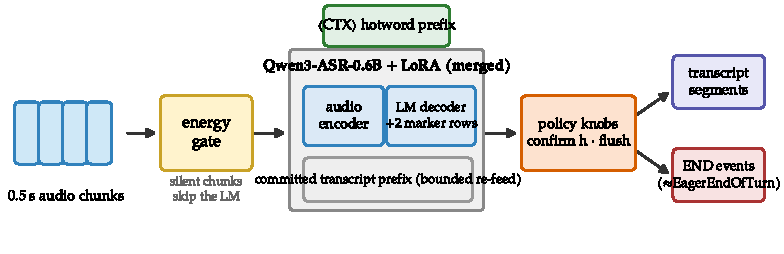
\includegraphics[width=\linewidth]{fig8_system}
  \caption{\textbf{System shape.} Audio chunks pass an RMS energy gate (silent chunks never start a segment, so mostly-silent sessions are nearly free); the merged LoRA model transcribes the current bounded segment with the \ctx{} hotword prefix in the system slot and may emit marker tokens; two policy knobs (confirm horizon, max-segment force-flush) sit \emph{behind} the model. Outputs are transcript segments plus END events --- the same event shape as Flux's \texttt{EagerEndOfTurn}.}
  \label{fig:system}
\end{figure}

\paragraph{Task.} A single-channel audio stream arrives in 0.5\,s chunks. At each chunk boundary the system must (a)~extend a running transcript and (b)~decide whether the turn has ended --- an irreversible, latency-sensitive event that downstream components act on. A text context prefix (user profile, hotword list) may be supplied at session start and should bias recognition throughout. We call the class \emph{turn-aware streaming ASR}: one model that transcribes while deciding, from semantics and silence jointly, whether the turn is over (Table~\ref{tab:matrix}).

\paragraph{Model.} We start from Qwen3-ASR-0.6B \citep{qwen3asr2026}, an open unified speech model (AuT audio encoder + dense Qwen3 decoder) with strong offline WER but no endpointing and no published context-biasing numbers. We claim two reserved vocabulary slots as marker tokens, \eager{} and \fire{}, and LoRA-fine-tune \citep{hu2022lora} the decoder ($r{=}16$, $\alpha{=}32$, q/k/v/o projections, plus the two marker embedding rows) to emit them inside the transcript at endpoint moments. Training data is ${\sim}12$k examples synthesized from LibriSpeech \citep{panayotov2015librispeech} and AMI \citep{carletta2005ami}; training takes hours on one GPU. \emph{Every model in this paper} --- the eight historical supervision recipes of \S\ref{sec:phantom} and the causal recipe of \S\ref{sec:relabel} --- shares this architecture, adapter recipe, data volume, and source corpora; the label specification is the only manipulated variable.

\paragraph{Inference policy.} Three orthogonal, interpretable knobs (Figure~\ref{fig:system}); every reported arm states its knob settings. The \textbf{energy gate} never \emph{starts} a segment on a silent chunk --- motivated by a data blind spot (\S\ref{sec:eval}), and also the serving trick that lets one engine carry many mostly-silent sessions (\S\ref{sec:serving}). The \textbf{confirm horizon} $h$ holds a fire candidate for $h$ further silent chunks before signaling END (resumed speech cancels the signal; the transcript flush stands) --- the phrase-vs-turn dial, which the causal model barely needs. The \textbf{max-segment force-flush} bounds the committed transcript segment; a transcription reset, never an END event.

\begin{table}[h]
  \centering\small
  \caption{The landscape. ``Cascade'' = VAD + silence timeout + separate ASR: the deployed default, and our measured baseline in Figure~\ref{fig:tradeoff}. Flux and \texttt{semantic\_vad} are the closed members of the turn-aware class this work opens.}
  \label{tab:matrix}
  \setlength{\tabcolsep}{3pt}
  \begin{tabular}{@{}lccccc@{}}
    \toprule
    & This work & Flux / \texttt{sem.vad} & Qwen3-ASR & Kyutai STT & Cascade \\
    \midrule
    Streaming ASR & \checkmark & \checkmark & \checkmark & \checkmark & \checkmark \\
    Semantic end-of-turn & \checkmark & \checkmark & --- & --- & timeout only \\
    Context biasing (numbers) & \checkmark\,($+28.9$\,pp) & --- & unreported & --- & ASR-dep. \\
    Open weights + recipe & \checkmark & --- & weights only & weights only & \checkmark \\
    \bottomrule
  \end{tabular}
\end{table}

\section{Anatomy of a phantom frontier}
\label{sec:phantom}

Eight supervision recipes were trained before the diagnosis; in hindsight the record reads like a controlled study of what contradictory supervision does to a model. We present it that way: first the symptoms as a function of supervision composition (\S\ref{sec:composition}), then the two label-side mechanisms (\S\ref{sec:mechanisms}), then the interventions that establish cause (\S\ref{sec:interventions}).

\subsection{Symptoms: a dose--response record}
\label{sec:composition}

Table~\ref{tab:composition} summarizes the eight-recipe sequence. Architecture, adapter recipe, data volume, and source corpora are fixed throughout; each row changes only the composition of the label pools. Three regularities stand out. First, every added pool moved the model \emph{along} an apparent frontier rather than off it: better streaming latency always arrived with worse offline fire recall, and vice versa --- so consistently that the record at the final row proposed shipping \emph{two} checkpoints, one per deployment. Second, the dose--response within a fix saturates: scaling the truncated-speech pool from 11\% to 38\% of the mix bought back only two of the thirteen seconds of premature firing, because the model was being asked to distinguish states that its labels made indistinguishable. Third, the terminal pathologies are qualitative, not quantitative: opposite labels on \emph{identical} audio collapsed the model to one side (row 5); opposite labels on \emph{disjoint but identically distributed} audio produced the bimodal training oscillation of Figure~\ref{fig:oscillation} (row 6). We return to that contrast in \S\ref{sec:interventions}.

\begin{table}[t]
  \centering\small
  \caption{\textbf{The supervision-composition record.} Eight recipes, one architecture; each row adds one labeled pool (cumulative). ``Early'' latencies are negative: the model fires seconds before the turn actually ends. The trade-off pattern --- every fix moves along the frontier, never off it --- is the second fingerprint of contradictory supervision.}
  \label{tab:composition}
  \setlength{\tabcolsep}{4pt}
  \begin{tabular}{@{}c>{\raggedright\arraybackslash}p{6.2cm}>{\raggedright\arraybackslash}p{6.4cm}@{}}
    \toprule
    \# & Supervision change (cumulative) & Observed behavior \\
    \midrule
    1 & offline endpoint pool only: fire at every clip end & fires eagerly and ``accurately'' offline (100\% fire recall); in streaming replay, fires 89$\times$ per speech-minute mid-utterance \\
    2 & $+$ truncated-speech hold pool (11\%${\to}$38\% of mix) & diminishing returns: median fire timing improves only $-13.1{\to}-9.6{\to}-7.6$\,s (still seconds early) as the dose rises \\
    3 & $+$ trailing-silence fire pool & streaming latency crosses zero (P50 $+0.32$\,s) \emph{but} offline fire recall regresses $100{\to}82$\%; the ``trade-off'' is first declared \\
    4 & $+$ complete utterances with \emph{and} without silence tails, both labeled fire & silence becomes optional again; a strictly intermediate point on the same frontier; frontier declared fundamental \\
    5 & $+$ hold pool on the \emph{same} audio as existing fire examples & collapse: opposite labels on identical inputs; the model stops firing on meeting audio entirely (fire recall 0\%) \\
    6 & $+$ hold pool on \emph{disjoint but identically distributed} audio & bimodal oscillation between fire-mode and no-fire-mode attractors for the whole run (Figure~\ref{fig:oscillation}, left); no checkpoint dominates; postmortem recommends shipping two checkpoints \\
    \midrule
    7 & \textbf{causal relabel (this work, \S\ref{sec:relabel}):} fire iff complete \emph{and} ${\ge}0.3$\,s observed silence & monotone training, both classes at ceiling simultaneously; single checkpoint dominates every predecessor (\S\ref{sec:results}) \\
    \bottomrule
  \end{tabular}
\end{table}

\subsection{The two mechanisms}
\label{sec:mechanisms}

Both of \S\ref{sec:clair}'s general mechanisms are present, and both inject opposite targets on causally identical prefixes (Figure~\ref{fig:contradictions}).

\begin{figure}[t]
  \centering
  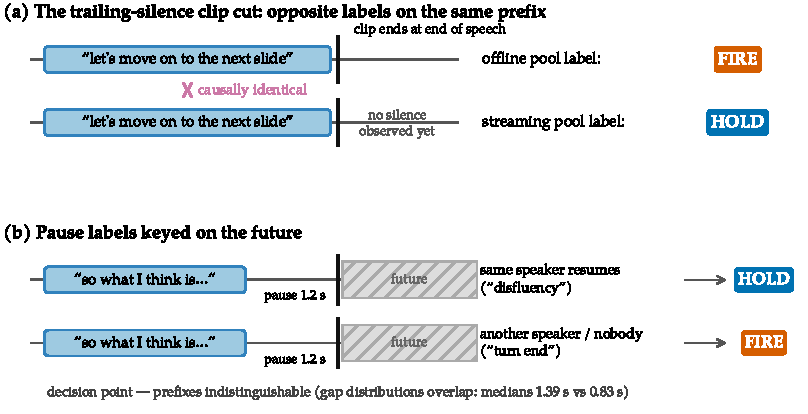
\includegraphics[width=\linewidth]{fig2_contradictions}
  \caption{\textbf{Two ways offline-derived supervision demands clairvoyance.} (a)~Offline clips inherit forced-alignment cuts at the end of speech, so the offline pool demands a fire on exactly the prefix the streaming pool labels \emph{hold} --- and the condition ``speech ended, no silence yet'' is one deployment never presents, because silence keeps arriving after a real speaker stops. (b)~Disfluency-vs-boundary pause labels are keyed on who speaks \emph{next}; at the decision point the prefixes are statistically indistinguishable (the two classes' silence-gap distributions overlap almost completely).}
  \label{fig:contradictions}
\end{figure}

\paragraph{The trailing-silence clip cut (Mechanism A).} Offline ASR clips end at the end of speech --- datasets are segmented by forced alignment, and evaluation clips inherit the cut. An offline endpoint benchmark built on such clips therefore demands a fire on audio that ends during or immediately after speech. The streaming pools (correctly) teach the opposite: never fire before silence is observed. The condition ``complete utterance, no trailing silence'' thus carries the label \emph{fire} in one pool and \emph{hold} in the other. In the opposed-pools recipe (Table~\ref{tab:composition}, row 6), the two pools were disjoint sets of AMI utterances with opposite labels on identically distributed content: 50/50 label noise on the exact decision the model exists to make.

\paragraph{Labels keyed on who speaks next (Mechanism B).} The historical pools separated ``disfluent pause --- hold'' from ``turn boundary --- fire'' using the transcript's segmentation: same speaker continues $\Rightarrow$ disfluency; another speaker follows $\Rightarrow$ boundary. Measured on the mixed-pools recipe's data, the two classes' silence-gap distributions overlap almost completely (medians 1.39\,s vs 0.83\,s). At decision time --- mid-pause --- the classes are indistinguishable; the label is a function of the future. An offline decoder can satisfy such labels by peeking; a causal model cannot, and part of the historical ``disfluency over-fire'' penalty punished models for lacking clairvoyance.

\subsection{Interventions: establishing cause}
\label{sec:interventions}

\paragraph{One second of silence falsifies the frontier.} If the offline benchmark's clip cut --- not any capability limit --- produced the fire-recall deficits, then restoring the future that deployment always delivers should erase them. It does. Appending 1.0\,s of silence to the offline evaluation clips, changing nothing else, takes the opposed-pools model's single-utterance fire recall from 0.10 to 1.00 and the mixed-pools model's from 0.82 to 0.98, while the offline-labeled model --- which never depended on hearing silence --- is the unchanged control (Table~\ref{tab:silappend}). Under deployment-realistic conditions all three models fire essentially perfectly on complete utterances: the entire single-utterance axis of the ``frontier,'' which four successive data recipes had been engineered against, was an artifact of where the evaluation clips ended.

\begin{table}[h]
  \centering\small
  \caption{\textbf{The silence-append intervention.} Fire recall on complete single utterances from the legacy offline benchmark, before and after appending 1.0\,s of silence to each clip. One evaluation-side variable erases the ``broken'' model's deficit; the offline-labeled model is the control.}
  \label{tab:silappend}
  \begin{tabular}{lccc}
    \toprule
    Model (supervision recipe) & original clips & $+1.0$\,s silence & $\Delta$ \\
    \midrule
    offline-labeled (row 1--2) & 1.00 & 1.00 & 0.00 \\
    mixed-pools (row 3) & 0.82 & 0.98 & $+0.16$ \\
    opposed-pools (row 6) & 0.10 & 1.00 & $+0.90$ \\
    \bottomrule
  \end{tabular}
\end{table}

\paragraph{Identical versus distributionally identical contradictions.} Rows 5 and 6 of Table~\ref{tab:composition} form a natural two-condition experiment on how a model \emph{expresses} a contradiction. When opposite labels sit on literally identical audio (row 5), the conflict is visible to the loss on every example and the model settles deterministically on one side --- it simply stops firing. When opposite labels sit on disjoint but identically distributed audio (row 6), no single example exposes the conflict; each pool is separately learnable, incompatible only in aggregate, and training \emph{circulates} between mode attractors that each satisfy one pool (Figure~\ref{fig:oscillation}, left). The oscillation is therefore not generic instability to be scheduled away; it is the loss surface reporting a contradiction that no example states outright.
%% TODO(exp-2): logit-level analysis of the oscillation — plot marker-token *probability*
%%   (not argmax accuracy) across the opposed-pools checkpoints. Distinguishes true mode
%%   circulation from threshold-flapping around p≈0.5; reviewers will ask.

\paragraph{The final intervention.} The remaining test is label-side: rebuild the pools under a causal rule, freeze everything else, and see whether both fingerprints vanish. They do (\S\ref{sec:relabel}); the resulting model's deployment behavior is quantified in \S\ref{sec:results}. First, however, we need an evaluation that cannot itself demand clairvoyance.

\section{Measuring what deployment sees}
\label{sec:eval}

If clairvoyant labels are the disease, evaluation is where it enters. We replaced both legacy benchmarks with one deployment-matched protocol --- and applied the causality principle to the benchmark itself.

\paragraph{Material and ground truth.} Continuous single-channel stretches from held-out AMI meetings: one target speaker's utterances at their true timeline offsets, silence between them, 30--60\,s per stretch (the voice-assistant shape: one microphone, one user; audio never ends at a speech boundary). Each utterance-end boundary is classified by what is observable \emph{on this channel}: \textbf{turn-final} (same-speaker gap ${\geq}2$\,s) --- should fire; \textbf{continuation} (gap in $[0.3,2)$\,s, same speaker resumes) --- firing is a measured segmentation \emph{cost} (\texttt{resume\_after\_fire}), not an error, because the correct answer depends on the future; \textbf{internal} (pauses inside utterances, or ${<}0.3$\,s after speech) --- firing is a \emph{false fire}. Metrics: boundary recall within $[-0.25,+1.5]$\,s, false fires per speech-minute, latency percentiles, resume rate, streaming WER of flushed transcripts, per-chunk compute.

\paragraph{The benchmark's own clairvoyant rule.} An early version of this benchmark promoted boundaries to turn-final when \emph{another meeting speaker} interleaved before the target speaker resumed --- speech that is inaudible on the replayed single channel. Demanding a fire there is exactly the clairvoyance the benchmark exists to remove; our own checklist (\S\ref{sec:checklist}) caught it. The corrected classification moved the mixed-pools model's recall $0.917{\to}0.906$ and the opposed-pools model's $0.935{\to}0.938$; no conclusion changed, but the episode is a working demonstration that evaluation pipelines inherit this failure mode as readily as training pipelines (details in Appendix~\ref{app:eval}).

\begin{figure}[t]
  \centering
  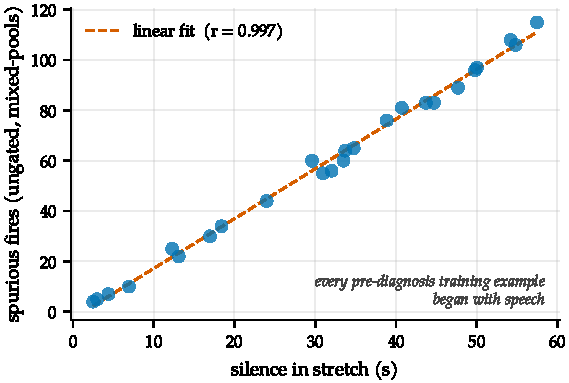
\includegraphics[width=0.62\linewidth]{fig6_silence}
  \caption{\textbf{Every clairvoyantly-supervised model is silence-incompetent.} Spurious fires of the ungated mixed-pools model against the silence content of each benchmark stretch: the model hallucinates text and sprays markers on silence at ${\sim}1.9$\,fires/s ($r=0.997$), because every pre-diagnosis training example begins with speech while a real channel is mostly silence (13 of 22 minutes here). Consequence: \emph{ungated} recall is uninterpretable --- a random 1.9\,Hz spammer scores 0.96 recall against the tolerance window. The fix costs one line (RMS energy gate), and the causal recipe additionally bakes silence schemas into training.}
  \label{fig:silence}
\end{figure}

\paragraph{Finding 1: silence incompetence.} Figure~\ref{fig:silence}. Every pre-diagnosis training example begins with speech; a real channel is mostly silence. On silence the models hallucinate and fire; ungated numbers are uninterpretable, and all comparisons below run gated.

\begin{figure}[t]
  \centering
  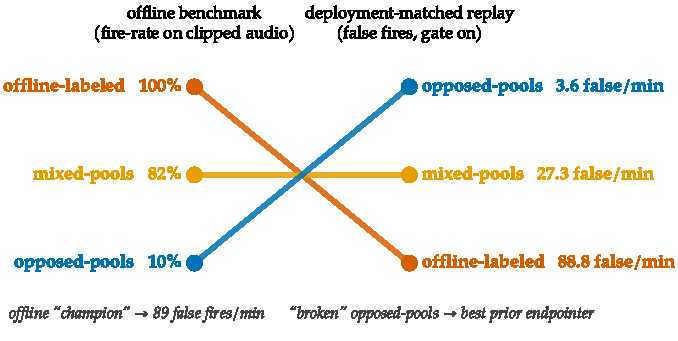
\includegraphics[width=0.62\linewidth]{fig5_inversion}
  \caption{\textbf{The ranking inversion.} Left: the legacy offline benchmark (fire-rate on clips cut at end-of-speech). Right: the deployment-matched replay benchmark (false fires per speech-minute, energy gate on; full metrics in Table~\ref{tab:main}). The offline champion fires 89 times per speech-minute mid-utterance --- its offline strength \emph{is} a premature-fire pathology once audio keeps flowing. The opposed-pools model, written off at 10\% offline, is the best prior endpointer. Both historical ship decisions were wrong.}
  \label{fig:inversion}
\end{figure}

\paragraph{Finding 2: the ranking inverts.} Figure~\ref{fig:inversion}. A benchmark with clairvoyant targets does not just mis-score models; it mis-\emph{ranks} them, and the error is largest exactly at the top --- the offline-labeled model was ``best'' offline \emph{because} it fires without waiting for silence, which is the single worst property in deployment.

\section{Relabel, don't rearchitect}
\label{sec:relabel}

The causal recipe changes only the data. One rule: \emph{emit \eager\fire{} at a point iff the speech so far is semantically complete AND ${\geq}0.3$\,s of silence has elapsed since the last speech.} Both conditions are functions of the prefix. Two corollaries kill the two contradictions. (1)~A complete utterance with no silence tail gets no marker --- and the \emph{same utterance} appears again with a silence tail and the marker (Figure~\ref{fig:minimalpair}): where the opposed-pools recipe assigned opposite labels to two pools of identically distributed audio (unlearnable), the causal recipe assigns opposite labels to the same audio differing only in an observable feature --- precisely the feature the model must learn to key on. (2)~Holding through a pause is trained only where the prefix itself says the utterance is incomplete (trailing filler/connective, mid-word cut); pauses after complete speech fire even if the speaker later resumes --- quick resumes become two segments, the benchmark's measured cost, not an error. Eight schemas cover fire, hold, truncation, pause discrimination, pure silence, and silence-initial segments (Appendix~\ref{app:labels}).
%% TODO(exp-3): schema ablation — causal recipe minus minimal pairs; minus silence schemas;
%%   minus incomplete-pause pool. Which component removes which symptom? Currently "only the
%%   labels changed" is true but unfactored; this is the reviewers' most likely ask.

\begin{figure}[t]
  \centering
  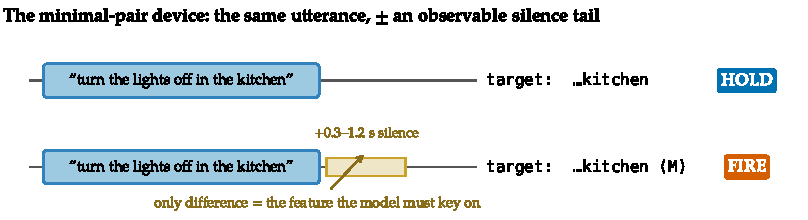
\includegraphics[width=\linewidth]{fig9_minimalpair}
  \caption{\textbf{The minimal-pair device.} Each complete utterance appears twice in the causal training data: without a silence tail (target: transcript only) and with a 0.3--1.2\,s tail (target: transcript + marker). The only difference between the opposite-labeled examples is the observable the model must use. This construction is what removes the oscillation in Figure~\ref{fig:oscillation}.}
  \label{fig:minimalpair}
\end{figure}

\paragraph{The fingerprint, removed.} Figure~\ref{fig:oscillation} (right): the composite climbs monotonically 0.900${\to}$0.963 and plateaus; fire and hold classes sit at ceiling simultaneously for the entire run. Architecture, recipe, scale, and sources held fixed --- as close to a controlled experiment on the label spec as a training run gets.

\section{Results}
\label{sec:results}

\begin{table}[t]
  \centering\small
  \caption{\textbf{Main result} (deployment-matched replay, energy gate on; latency-vs-false-fire view in Figure~\ref{fig:tradeoff}). Rows 1--4: the 25-stretch development benchmark (96 turn-final boundaries). The causal model dominates every predecessor without either crutch: its \emph{raw} false-fire rate beats the mixed-pools model's \emph{confirmed} rate, and its WER needs no force-flush. The confirm ablation: the mixed-pools horizon cancels 241 phrase-boundary candidates; the causal model's cancels 3. Last row: a \emph{fresh} $2\times$-larger stretch set (50 stretches, 184 boundaries) drawn after all development ended --- latency and false fires hold; recall dips 4.5\,pp (\S\ref{sec:limits}). $^{\dagger}$WER mean dominated by long-monologue repetition loops when no force-flush bounds the segment (causal fresh-set WER \emph{median} 0.30, matching the development set; the \S\ref{sec:serving} force-flush bounds this tail).}
  \label{tab:main}
  \begin{tabular}{lccccc}
    \toprule
    Policy & Recall\,$\uparrow$ & P50\,$\downarrow$ & P95\,$\downarrow$ & False/min\,$\downarrow$ & WER$_\text{mean}$\,$\downarrow$ \\
    \midrule
    mixed-pools + gate + confirm $h{=}1$ & 0.927 & 0.68\,s & 1.27\,s & 3.2 & 0.36 \\
    opposed-pools + gate + confirm $h{=}1$ & 0.938 & 0.77\,s & 1.06\,s & 0.0 & 4.96$^{\dagger}$ \\
    \textbf{causal + gate (ours)} & \textbf{0.969} & \textbf{0.39\,s} & \textbf{0.70\,s} & \textbf{0.3} & \textbf{1.43} \\
    causal + gate + confirm $h{=}1$ & 0.969 & 0.89\,s & 1.20\,s & 0.0 & 1.43 \\
    causal + gate --- fresh 50-stretch set & 0.924 & 0.42\,s & 0.70\,s & 0.2 & 4.63$^{\dagger}$ \\
    \bottomrule
  \end{tabular}
\end{table}

\begin{figure}[t]
  \centering
  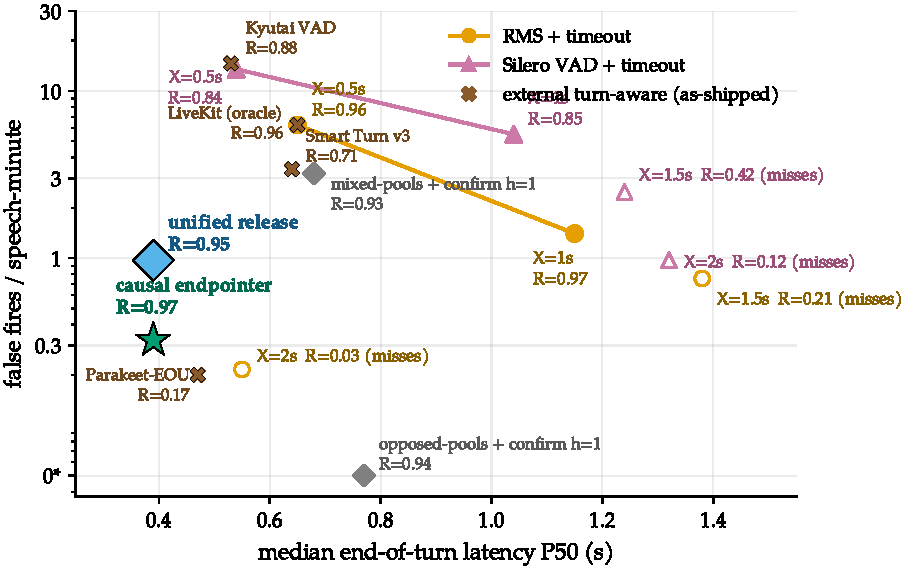
\includegraphics[width=0.72\linewidth]{fig3_tradeoff}
  \caption{\textbf{Semantic endpointing escapes the timeout curve.} Median latency vs false fires (log scale; $0^{*}$ = zero plotted at $0.05$) on identical stretches, detector, and scoring. A silence timeout $X$ can only slide along its curve: matching the causal model's recall takes $X{=}1.0$\,s --- $3\times$ the latency, ${\sim}5\times$ the false fires; the fastest usable setting ($X{=}0.5$\,s) produces $21\times$ the false fires; $X{\geq}1.5$\,s leaves the recall tolerance window entirely (open markers) --- the assistant that waits too long. The Silero cascade \citep{silero2021vad} is dominated by plain RMS on this close-talk channel. The causal model sits strictly inside the whole family because it reads \emph{completeness}: it fires 0.39\,s after a finished thought and holds through a 1.4\,s mid-sentence pause. Honest caveat: it segments quick resumes at the same rate as an aggressive timeout (resume-after-fire 1.0, by design --- the correct choice is unknowable at decision time); deployments preferring merged segments pay $+0.5$\,s via confirm $h{=}1$.}
  \label{fig:tradeoff}
\end{figure}

\paragraph{Dominance.} Table~\ref{tab:main} and Figure~\ref{fig:tradeoff}. Against its predecessors, the causal model with the gate alone is better on every axis at once. Against the deployed cascade, the comparison's \emph{structure} is the point: a timeout must be long enough to survive within-turn pauses, so it can only trade latency against false fires along one curve; the causal model escapes the curve by reading completeness. And the crutches retire: the phrase-vs-turn discrimination moved from inference policy into weights --- which is what supervision was supposed to do all along.
%% TODO(exp-4): external baselines on this benchmark — Smart Turn, LiveKit's turn detector
%%   (text-based, fed the streaming transcript), Kyutai's semantic-VAD head. Timeout cascades
%%   alone invite the "you only beat the strawman" review.

\paragraph{Held-out confirmation and uncertainty.} The 25-stretch development benchmark was reused across development, so we drew a fresh $2\times$-larger set (50 stretches, 184 turn-final boundaries) after all development ended. Latency, false fires, and WER median reproduce; recall drops $0.969 \to 0.924$. The 95\% Wilson intervals --- $[0.91, 0.99]$ on the development set (93/96) and $[0.88, 0.95]$ on the fresh set (170/184) --- overlap, so the drop is within sampling variation, though its direction is consistent with mild adaptive overfitting to the development set. We treat the fresh set as the honest operating estimate. Read against the same-set timeout family (Appendix~\ref{app:tables}): the cascade can reach higher recall on this set (0.978--0.989 at $X{\in}\{0.5,1.0\}$\,s) but only at $1.7$--$2.9\times$ the causal model's latency and $3$--$22\times$ its false fires --- and no timeout setting reaches the causal model's $(0.42\,\text{s},\,0.21/\text{min})$ corner at \emph{any} recall.

\section{The rest of the model still works}
\label{sec:capability}

An endpoint fine-tune that damaged the base recognizer would be a bad trade. It does not --- and the unified model's side capability comes with numbers its base model never published.

\paragraph{Offline ASR regression --- measured and attributed.} Table~\ref{tab:wer}: the endpoint fine-tune costs $+1.1$\,pp WER on LibriSpeech test-clean and $+2.7$\,pp on test-other. Our first hypothesis was mechanical: the model fires its marker on 4.7--5.9\% of offline clips (many LibriSpeech clips carry the ${\geq}0.3$\,s silence tail where the causal rule \emph{says} fire), and a fire ends the decode, truncating the transcript. We tested it by banning the two marker tokens at decode time --- and the hypothesis \emph{fails}: fires drop to zero, WER does not move (3.94\%/7.91\%). The regression is genuine distributional drift from fine-tuning on ${\sim}12$k narrow-schema examples with no plain-ASR replay data, and the standard mitigation (mixing transcription-only data into the fine-tune) is unexercised in this release. The deployment-relevant \emph{streaming} WER is unaffected (Table~\ref{tab:main}, median 0.28--0.30 across sets), so the cost is confined to using the endpoint checkpoint as an offline transcriber --- a job the base checkpoint still does.

\begin{table}[h]
  \centering\small
  \caption{\textbf{Offline WER regression} (LibriSpeech, full official splits, single-shot decode on vLLM, jiwer/whisper normalization). ``Fires'' = fraction of clips where the model emitted the endpoint marker (offline clips end at or near end-of-speech; base never fires because its marker rows are untrained).}
  \label{tab:wer}
  \begin{tabular}{lcccc}
    \toprule
    & \multicolumn{2}{c}{WER\,$\downarrow$} & \multicolumn{2}{c}{Fires} \\
    \cmidrule(lr){2-3}\cmidrule(lr){4-5}
    Model & clean & other & clean & other \\
    \midrule
    Qwen3-ASR-0.6B (base) & 2.79\% & 5.14\% & 0\% & 0\% \\
    + endpoint LoRA (merged, causal) & 3.93\% & 7.87\% & 4.7\% & 5.9\% \\
    + markers banned at decode & 3.94\% & 7.91\% & 0\% & 0\% \\
    \bottomrule
  \end{tabular}
\end{table}

\paragraph{Context biasing, measured where it matters.} Figure~\ref{fig:biasing}(a): on Earnings-22 \citep{delrio2022earnings22} --- spontaneous earnings-call speech dense in tickers, executives, products; entities LLM-extracted and filtered to genuine proper nouns --- a relevant hotword prefix lifts entity recall from 66.7\% to 95.6\% ($+28.9$\,pp), while nudging WER down (15.3${\to}$15.0\%). A \emph{distractor} prefix (another utterance's entities) induces 3.7\% hallucination --- above our 3\% target, reported as-is; distractor-ratio training is the known, unexercised lever. Qwen3-ASR claims context biasing but reports no numbers; to our knowledge these are the first on this model family.

\paragraph{The advantage survives session length.} Figure~\ref{fig:biasing}(b): with 0--12\,s of unrelated speech interposed between the prefix and the target words, the biasing advantage stays flat at ${\approx}{+}30$\,pp. Context biasing is a durable session-level capability, not a first-utterance parlor trick.

\begin{figure}[t]
  \centering
  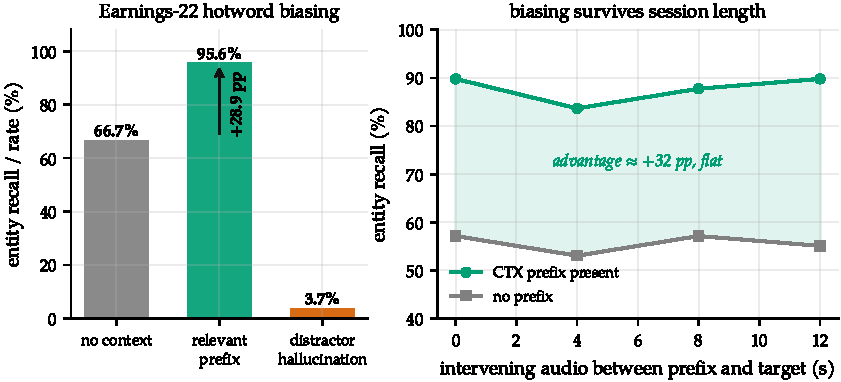
\includegraphics[width=\linewidth]{fig4_biasing}
  \caption{\textbf{Context biasing: the capability with no public numbers.} (a)~Earnings-22 entity recall without context, with the relevant hotword prefix, and the hallucination rate under a distractor prefix (150 utterances; LLM-extracted proper-noun entities). (b)~Recall vs seconds of unrelated speech interposed between prefix and target: the ${\approx}{+}30$\,pp advantage does not decay with session age.}
  \label{fig:biasing}
\end{figure}

\section{Deployment reality check}
\label{sec:serving}

Streaming papers routinely stop at a simulator; we serve the model on stock vLLM \citep{kwon2023vllm} on one \emph{shared} GPU and report three findings in brief (full details and figure in Appendix~\ref{app:serving}). First, an out-of-distribution landmine: the natural flat-cost serving shape --- appending each 0.5\,s chunk as a new audio placeholder in a growing resident request --- destroys the model (88\% WER vs 3.8\% for re-feeding the last window as a single segment), because the base model was trained on single audio segments; bounded re-feed is the only correct primitive for this family. Second, the simulator was the bottleneck: the replay protocol on vLLM reproduces the endpoint behavior at 84\,ms median per 0.5\,s chunk versus the transformers simulator's 455\,ms ($5.4\times$) --- latency claims made on $O(T^2)$ re-decode simulators overstate the cost of this approach by that factor. Third, bound every resident state: a 20\,s max-segment force-flush fixes both the long-monologue WER tail (2.54${\to}$1.29) and the compute tail (P95 413${\to}$117\,ms) at no endpoint cost, and per-frame P95 stays flat through $N{=}8$ concurrent sessions per 0.15-GPU slice --- deadline-bound, not memory-bound. The in-engine efficiency variant --- windowed KV with the \ctx{} prefix pinned as an attention sink \citep{xiao2024streamingllm} --- is validated separately in a companion systems paper \citep{li2026metronome}.

\section{Clairvoyant labels: a checklist}
\label{sec:checklist}

The failure mode generalizes to any model that must act mid-stream on offline-labeled data. Four questions for a streaming supervision pipeline:

\begin{tcolorbox}[colback=blue!3!white,colframe=blue!45!black,title=\textbf{Is your supervision clairvoyant?}]
\begin{enumerate}\itemsep2pt
  \item \textbf{Prefix test.} For each label at decision time $t$: is it computable from input up to $t$? \emph{(Our pause labels were keyed on the next speaker.)}
  \item \textbf{Twin test.} Can two causally identical prefixes receive different labels anywhere in the data? \emph{(Same complete-utterance prefix: fire in one pool, hold in the other.)} Minimal pairs differing in an \emph{observable} are the fix, not the bug.
  \item \textbf{Phantom-condition test.} Does the eval demand behavior on conditions deployment never produces? \emph{(Clips cut at end-of-speech; deployment always delivers the next silence.)}
  \item \textbf{Oscillation test.} Does training bounce between mode attractors that each satisfy part of the data? That is not instability to be scheduled away; it is the loss surface reporting a contradiction.
\end{enumerate}
\end{tcolorbox}

Candidates we believe are affected: turn-taking policies for full-duplex agents trained from offline dialogue transcripts (the labels encode who \emph{did} speak next, not what was knowable --- cf.\ the projection-style objectives of \citealp{ekstedt2022vap}, which are explicitly predictive and thus honest about the uncertainty); barge-in and endpointing in commercial stacks; simultaneous translation trained with reference-aligned read/write decisions \citep{ma2019stacl}; streaming TTS interruption; tool-call timing for agents cloned from completed trajectories --- a streaming sibling of causal confusion in imitation learning \citep{dehaan2019causal}. In each, an apparent aggressiveness-vs-caution frontier may partly be an artifact of asking the model to know the future. The diagnosis also joins a broader lineage of measurement-induced phenomena: as sharp metric choices can manufacture ``emergence'' \citep{schaeffer2023mirage}, non-causal label choices can manufacture \emph{trade-offs}.

\section{Related work}
\label{sec:related}

\paragraph{Endpointing and end-of-turn detection.} Classical endpointing thresholds a VAD \citep{silero2021vad} with a silence timeout; learned refinements predict end-of-query directly from acoustics \citep{shannon2017improved}, jointly train an endpointer with the recognizer \citep{chang2019joint,li2020towards,bijwadia2023unified}, or distill tiny acoustic end-of-turn models \citep{helwani2026hierarchical,smartturn2025}. Recent systems fuse acoustic and linguistic cues for the turn decision \citep{fastturn2026,jalturn2026} or fold VAD, turn detection, and ASR into one audio-LLM front-end \citep{uaf2026}. Commercially, Deepgram Flux integrates end-of-turn events into the recognizer's forward pass \citep{deepgram2026flux} and OpenAI exposes semantic VAD \citep{openai2025semanticvad}; neither publishes training details. Our contribution to this line is orthogonal to architecture: a supervision principle, with evidence that violating it manufactures the recall-precision trade-offs this literature often reports as intrinsic.

\paragraph{Turn-taking in dialogue.} Turn-taking prediction has a long tradition in conversational AI \citep{skantze2021review}, from text-based end-of-turn prediction \citep{ekstedt2020turngpt} to voice-activity projection trained on future windows \citep{ekstedt2022vap}. Projection objectives predict distributions over the future and are therefore causally honest; our diagnosis concerns the sharper failure where future-dependent quantities are presented as \emph{deterministic labels}.

\paragraph{Streaming and unified ASR.} Streaming recognition spans RNN-T \citep{graves2012sequence}, large weakly supervised models \citep{radford2023whisper}, decoder-only streaming with latency losses \citep{wan2026streaming}, and unified streaming/offline speech-LLMs \citep{qwen3asr2026}. Kyutai's delayed-streams models add a semantic-VAD head to streaming STT \citep{kyutai2025stt,defossez2024moshi}. We inherit this substrate and add the turn event plus the training recipe.

\paragraph{Context biasing.} Contextual ASR ranges from attention-based deep context \citep{pundak2018deep} to retrieval-scale biasing \citep{brasr2025}, RL-tuned hotword integration \citep{hotwordgrpo2025}, and cue-based prompting for speech LLMs \citep{commoncues2026}. We use plain prompt-slot biasing and contribute measurements: uplift on entity-dense audio and durability across session age.

\paragraph{Serving.} vLLM's paged KV \citep{kwon2023vllm} carries our serving path; attention sinks \citep{xiao2024streamingllm} and bounded-state streaming serving \citep{li2026metronome} provide the in-engine efficiency variant of our pinned context prefix.

\section{Limitations}
\label{sec:limits}

The case study is single-speaker, single-channel English; the mixed-channel meeting shape is future work. Each supervision recipe in Table~\ref{tab:composition} was trained once: the oscillation-versus-monotone contrast of Figure~\ref{fig:oscillation} rests on one run per condition, and multi-seed replication --- along with a component-wise ablation of the causal recipe (minimal pairs, silence schemas, incomplete-pause pool) --- is the immediate next step before the mechanism claim can be considered settled. Semantic completeness labels come from a heuristic transcript classifier (fillers, connectives, short-utterance rules); a learned completeness judge is the obvious next lever on the residual recall gap. Distractor hallucination (3.7\%) exceeds our 3\% target. Quick resumes are always segmented (resume rate 1.0); merging them costs $+0.5$\,s via the confirm knob or requires post-hoc fusion. Concurrency numbers are contention-caveated lower bounds from a shared GPU. The development benchmark was reused across development; the fresh-set recall (0.924, overlapping Wilson intervals, \S\ref{sec:results}) is the honest operating estimate. The endpoint fine-tune costs offline WER (\S\ref{sec:capability}): mixing plain ASR data into the fine-tune is the standard, unexercised mitigation.

% ════════════════════════════════════════════════════════════
\section*{Acknowledgements}
% ════════════════════════════════════════════════════════════

We thank Mingqi Yang from Minimax AI for early discussions.
This paper was produced using Pine Copilot's voice-directed \emph{whisper coding} workflow~\citep{pineai2026whispercoding}, in which the authors specify, discuss, and review the work by voice while a coding agent---Claude Code with Claude Opus 4.8---carries out the planning, coding, experiments, and paper writing.
We thank BSQL Networking for hosting the NVIDIA RTX PRO 6000 GPU.

\bibliographystyle{plainnat}
\bibliography{refs}

\clearpage

\appendix

\section{The causal label specification}
\label{app:labels}
Eight schemas, ${\sim}12$k examples, LibriSpeech and AMI roughly 50/50; pair examples use both same- and different-speaker AMI pairs (the fire decision keys on completeness + silence, never on speaker identity, which single-channel deployment cannot observe). $M$ = \eager\fire.

\begin{table}[h]
  \centering\small
  \caption{Causal training schemas. Schemas 1--2 are the minimal-pair device (Figure~\ref{fig:minimalpair}); 7--8 fix silence incompetence (Figure~\ref{fig:silence}).}
  \begin{tabular}{lll}
    \toprule
    \# & Construction & Target \\
    \midrule
    1 & complete utterance + 0.3--1.2\,s silence tail & \texttt{text} $M$ \\
    2 & \emph{same utterances as \#1}, tail ${\leq}0.1$\,s & \texttt{text} \\
    3 & speech truncated mid-utterance at 30--80\% & partial \texttt{text} \\
    4 & complete A + gap 0.3--2.5\,s + B (+ tail) & \texttt{A} $M$ \texttt{B} $M$ / \texttt{A} $M$ \texttt{B} \\
    5 & \emph{incomplete} A + gap + B + tail & \texttt{A B} $M$ \\
    6 & complete utterance + long silence (2--4\,s) & \texttt{text} $M$ \\
    7 & pure silence 0.5--4\,s & (empty) \\
    8 & leading silence 0.5--2\,s + utterance + tail & \texttt{text} $M$ \\
    \bottomrule
  \end{tabular}
\end{table}

Completeness classifier for pair examples: utterance A is \emph{incomplete} iff its transcript ends in a filler/connective (``and, but, so, or, uh, um, the, a, to, of, in, with, i mean, you know, \ldots''), ends mid-word (AMI partial-word annotation), or has fewer than 3 words outside a closed acknowledgment list. Borderline cases land in the \texttt{resume\_after\_fire} cost knob --- they never create fire/hold contradictions on identical observables. Abandonment (incomplete speech, speaker never resumes) is an inference-policy timeout, not a label.

\section{Benchmark specification and the corrected classifier}
\label{app:eval}
Full protocol: 0.5\,s chunks; committed-prefix incremental decoding (emitted text committed, last 5 tokens rolled back) matching the base model's official streaming semantics; fires timestamped at the chunk boundary where \fire{} first appears; recall window $[-0.25,+1.5]$\,s clipped at the next utterance's onset. The first version of the boundary classifier promoted a boundary to turn-final when another meeting speaker interleaved before the target speaker resumed. On a single-channel stream that speech is silence --- demanding a fire there is exactly the clairvoyance the benchmark exists to remove. The corrected classification moved the mixed-pools model's recall $0.917{\to}0.906$ and the opposed-pools model's $0.935{\to}0.938$; no conclusion changed, but the episode is a working example of \S\ref{sec:checklist} applied to one's own evaluation.

\section{Additional results}
\label{app:tables}

\paragraph{Gated arms and the confirm-horizon sweep.} Table~\ref{tab:appconfirm}. The confirm horizon behaves as a clean latency-vs-false-fire dial: $h{=}1$ strictly improves the mixed-pools model (recall \emph{rises} because deferring the fire lets the segment gather the boundary inside tolerance) and zeroes the opposed-pools and causal models' false fires; $h{=}2$ over-suppresses (mixed-pools recall 0.812, latency past budget). The causal model is the only checkpoint whose $h{=}0$ row is already deployable. Ungated arms are omitted as uninterpretable (Figure~\ref{fig:silence}): with ${\sim}1.9$ spurious fires per second on silence, the pre-diagnosis models score 0.95--0.99 ``recall'' by chance; their gated rows below are the meaningful ones.

\begin{table}[h]
  \centering\small
  \caption{All gated arms on the 25-stretch development benchmark. Resume = \texttt{resume\_after\_fire} rate over continuation boundaries (a cost knob, not an error rate).}
  \label{tab:appconfirm}
  \begin{tabular}{lcccccc}
    \toprule
    Arm & Recall & P50 & P95 & False/min & Resume & WER$_\text{mean}$ \\
    \midrule
    offline-labeled + gate & 0.896 & 0.05\,s & 0.25\,s & 88.8 & 0.89 & 0.85 \\
    mixed-pools + gate & 0.906 & 0.16\,s & 0.89\,s & 27.3 & 0.96 & 0.36 \\
    mixed-pools + gate + confirm $h{=}1$ & 0.927 & 0.68\,s & 1.27\,s & 3.2 & 0.85 & 0.36 \\
    mixed-pools + gate + confirm $h{=}2$ & 0.812 & 1.15\,s & 1.42\,s & 1.1 & 0.56 & 0.36 \\
    opposed-pools + gate & 0.938 & 0.26\,s & 0.56\,s & 3.6 & 0.93 & 4.96 \\
    opposed-pools + gate + confirm $h{=}1$ & 0.938 & 0.77\,s & 1.06\,s & 0.0 & 0.85 & 4.96 \\
    causal + gate & 0.969 & 0.39\,s & 0.70\,s & 0.3 & 1.00 & 1.43 \\
    causal + gate + confirm $h{=}1$ & 0.969 & 0.89\,s & 1.20\,s & 0.0 & 0.93 & 1.43 \\
    \bottomrule
  \end{tabular}
\end{table}

\paragraph{The full timeout family.} Table~\ref{tab:apptimeout}, both detectors on the development (25 stretches) and fresh confirmation (50 stretches) sets. The family's shape is stable across sets: recall collapses between $X{=}1.0$ and $1.5$\,s (the fire lands outside the $+1.5$\,s tolerance), and no setting reaches the causal model's (recall, latency, false-fire) point. Silero ran per-chunk with state resets --- a slight handicap noted in \S\ref{sec:results}; RMS shares the LM arms' exact detector and is the apples-to-apples policy comparison.

\begin{table}[h]
  \centering\small
  \caption{Silence-timeout cascade, all settings, on the development (dev) and fresh confirmation (conf) stretch sets.}
  \label{tab:apptimeout}
  \begin{tabular}{llcccccc}
    \toprule
    Detector & Set & $X$ (s) & Recall & P50 & P95 & False/min & Resume \\
    \midrule
    RMS & dev & 0.5 & 0.958 & 0.65\,s & 0.94\,s & 6.3 & 1.00 \\
    RMS & dev & 1.0 & 0.969 & 1.15\,s & 1.44\,s & 1.4 & 0.81 \\
    RMS & dev & 1.5 & 0.208 & 1.38\,s & 1.49\,s & 0.8 & 0.07 \\
    RMS & dev & 2.0 & 0.031 & 0.55\,s & 0.55\,s & 0.2 & 0.00 \\
    RMS & conf & 0.5 & 0.978 & 0.70\,s & 0.95\,s & 4.6 & 0.99 \\
    RMS & conf & 1.0 & 0.989 & 1.20\,s & 1.45\,s & 0.6 & 0.73 \\
    RMS & conf & 1.5 & 0.185 & 1.44\,s & 1.50\,s & 0.4 & 0.07 \\
    RMS & conf & 2.0 & 0.016 & 1.14\,s & 1.14\,s & 0.2 & 0.00 \\
    Silero & dev & 0.5 & 0.844 & 0.54\,s & 0.88\,s & 13.5 & 0.96 \\
    Silero & dev & 1.0 & 0.854 & 1.04\,s & 1.38\,s & 5.5 & 0.85 \\
    Silero & dev & 1.5 & 0.417 & 1.24\,s & 1.49\,s & 2.5 & 0.41 \\
    Silero & dev & 2.0 & 0.125 & 1.32\,s & 1.42\,s & 1.0 & 0.00 \\
    Silero & conf & 0.5 & 0.837 & 0.51\,s & 0.83\,s & 12.3 & 0.88 \\
    Silero & conf & 1.0 & 0.864 & 1.00\,s & 1.33\,s & 4.4 & 0.73 \\
    Silero & conf & 1.5 & 0.451 & 1.29\,s & 1.48\,s & 2.0 & 0.27 \\
    Silero & conf & 2.0 & 0.130 & 1.34\,s & 1.44\,s & 1.3 & 0.07 \\
    \bottomrule
  \end{tabular}
\end{table}

\paragraph{Fresh-set confirmation.} The causal model with the gate on the confirmation set: recall 0.924, P50 0.42\,s, P95 0.70\,s, 0.21 false fires/min, resume 0.91, WER median 0.30 / mean 4.63 (three long-monologue stretches enter the no-flush repetition loop; the \S\ref{sec:serving} force-flush is the documented fix). The 4.5\,pp recall drop from the development set is the generalization gap discussed in \S\ref{sec:results} and \S\ref{sec:limits}.

\section{Serving details}
\label{app:serving}

\begin{figure}[h]
  \centering
  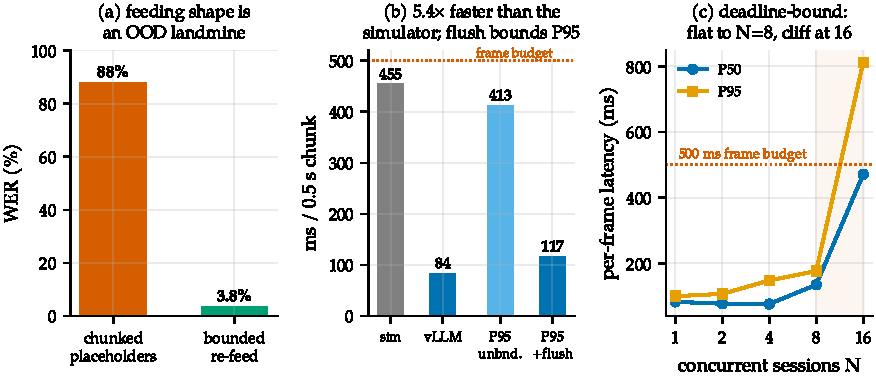
\includegraphics[width=\linewidth]{fig7_serving}
  \caption{\textbf{Serving on real infrastructure.} (a)~Feeding shape: per-chunk audio placeholders are out-of-distribution for a model trained on single segments (88\% WER); bounded re-feed of the last window costs a re-encode but is correct (3.8\%). (b)~Per-chunk compute: the vLLM path is $5.4\times$ faster than the transformers simulator used for all pre-serving latency numbers; the max-segment force-flush also bounds the P95 tail. (c)~Concurrent sessions per engine on a 0.15-GPU slice: flat to $N{=}8$, cliff at 16 --- the deadline binds, not memory.}
  \label{fig:serving}
\end{figure}

Figure~\ref{fig:serving} shows the three findings of \S\ref{sec:serving}. (a)~The natural flat-cost serving shape --- appending each 0.5\,s chunk as a new audio placeholder in a growing resident request --- destroys the model: 88\% WER vs 3.8\% for re-feeding the last window as a single segment. The base model was trained on single audio segments; per-chunk placeholders are wildly out of distribution. Bounded re-feed is the only correct primitive for this family. (b)~The replay protocol on vLLM reproduces the endpoint behavior at 84\,ms median per chunk vs the transformers simulator's 455\,ms ($5.4\times$) --- ${\sim}6\times$ real time on a 0.15-utilization slice. (c)~Unbounded committed prefixes eventually loop on long monologues; a 20\,s force-flush fixes the WER tail (2.54${\to}$1.29) \emph{and} the compute tail (P95 413${\to}$117\,ms) at no endpoint cost. Under concurrency, per-frame P95 stays flat through $N{=}8$ sessions per 0.15-GPU slice and cliffs at 16 --- deadline-bound, not memory-bound, with the energy gate batching only the sessions actually due each frame (a contention-caveated lower bound; the shape, not the constant, is the result).

\section{Reproducibility}
\label{app:repro}
Hardware: one RTX Pro 6000 (Blackwell), shared with an unrelated co-tenant workload throughout (all GPU jobs wrapped in retry/resume; the causal training run survived four OOM kills via checkpoint resume with ${\leq}750$ steps lost each). Training: LoRA $r{=}16$, $\alpha{=}32$, batch 8, best checkpoint at step 7.5k selected by the holdout composite. Evaluation and serving: vLLM 0.19, \texttt{skip\_special\_tokens=False} (the markers are reserved special tokens and are otherwise silently stripped --- a gotcha worth one sentence). Code, the label-spec builder, the replay benchmark, and the merged checkpoint are released at \url{https://github.com/19PINE-AI/turn-aware-asr}; the repository README documents the mapping from its internal checkpoint directory names to the supervision recipes described in this paper.

\end{document}
